%\documentclass[10pt]{article}\usepackage[correction,nu]{esial}
\documentclass[10pt]{article}\usepackage[nu]{esial}
\usepackage{amstext,amsmath,amsfonts}
\TOP\1A
\newcommand{\WP}[1]{\textbf{WP}($#1$)}

\usepackage{amsthm,pifont,textcomp}
\usepackage{amsmath,amssymb}

\usepackage[utf8]{inputenc}
\graphicspath{{fig/}}

\begin{document}
\title{Examen du 6/03/2010 (2h)}
\fvset{fontsize=\footnotesize}
\maketitle

\begin{centering}
  \textbf{\large Documents interdits, à l'exception d'une feuille A4 à rendre
    avec votre copie.}

\end{centering}
\centerline{La notation tiendra compte de la présentation et de la clarté de
  la rédaction.}
\bigskip



\bigskip\QuestionCours~(4pt)

\Question(1pt) Quelle est la différence entre la complexité dans le pire
cas et la borne supérieure de complexité?

\begin{Reponse}
  La borne supérieure de complexité ($O(n)$) est une approximation
  asymptotique, donc cela sert à étudier le comportement de la fonction quand
  le paramètre devient grand. La complexité dans le pire cas est une réflexion
  menée pour une valeur du paramètre donnée. On cherche alors la pire instance
  du problème pour mettre l'algorithme en difficulté. 

  Par exemple, pour le tri à bulle, le pire cas est quand le tableau est trié
  dans l'ordre inverse et il va effectuer un nombre de swaps de l'ordre de
  $n^2$ (et $n$ parcours), tandis que le meilleur cas est quand le tableau est
  déjà trié. Dans ce cas, il fait un seul parcours et aucun swap. 

  Mais si la complexité de ce tri est notée TB, on a $TB(n)\in O(n^2)$, ce qui
  veut dire que quand $n$ est suffisament grand, $TB(n)$ n'est jamais pire que
  $n^2$ (aux constantes près).
\end{Reponse}

\Question(1pt) Définissez les types de récursivité suivants: terminale,
générative, mutuelle (ou croisée) et structurelle.

\begin{Reponse}
  \begin{itemize}
  \item \textbf{Terminale:} aucune opération n'a lieu lors de la remontée
    récursive
  \item \textbf{Générative:} c'est une fonction qui est récursive (par
    opposition à structurelle)
  \item \textbf{Mutuelle:} deux (ou plus) fonctions s'appellent les unes les
    autres
  \item \textbf{Structurelle:} c'est une structure de données qui est récursive
    (par opposition à générative)
  \end{itemize}
\end{Reponse}

\Question(1pt) Qu'est ce que le backtracking?

\begin{Reponse}
  C'est une technique algorithmique permettant d'effectuer des recherches
  combinatoires bien plus efficacement qu'un parcours exaustif. L'idée de base
  est de construire peu à peu les solutions en ne parcourant que des
  sous-solutions valides. Dès qu'une sous-solution est invalide, on arrête
  l'exploration de cette branche, ce qui permet d'éviter le parcours de
  nombreuses solutions complètes qui seraient invalidées par la présence de la
  sous solution courante. Ouf.
  
  Pour mettre en œuvre le backtracking, on utilise généralement une récursion
  (pour construire peu à peu la solution) avec une boucle ou similaire pour
  parcourir tous les choix possibles à une étape donnée de la construction de
  notre solution. Pour chaque choix, s'il mène à une sous-solution valide
  également, on opère un appel récursif pour explorer les sous-solutions plus
  grandes que l'on peut construire avec celle que l'on a pour l'instant. 
\end{Reponse}

\ifcorrection{\newpage}{}

\Question(1pt) Définissez les tests (1) white box (2) black box (3)
d'intégration (4) de régression.

\begin{Reponse}
  \begin{itemize}
  \item \textbf{Whitebox:} C'est une technique de tests, une facon d'imaginer
    les tests à faire pour remplir mes objectifs; J'écris mes tests en lisant
    le source (et je teste donc les cas limites de l'implémentation)
  \item \textbf{Blackbox:} C'est également une technique de tests; je n'ai que
    la spécification pour écrire les tests (et j'ai donc moins de matière
    puisque je ne sais pas comment sont représentés les choses)
  \item \textbf{Intégration:} C'est une stratégie de tests, un objectif à
    remplir par une batterie de tests. C'est quand j'ai plusieurs modules
    (peut-être testés chacun par tests unitaires) et que je veux m'assurer que
    tous fonctionnent correctement ensemble, qu'il n'y a pas de problème aux
    interfaces lors de la composition.
  \item \textbf{Regression:} Quand j'ai trouvé une erreur (un bug) dans mon
    programme, je dois écrire un test cherchant à le reproduire afin de
    m'assurer que ce bug ne refera pas surface lors d'une modification
    ultérieure du code. 
  \end{itemize}
\end{Reponse}

\bigskip\Exercice\textbf{Code récursif mystère} (5pt). 

Considérez le code mystère suivant. 

\noindent\begin{minipage}{.65\linewidth}

\Question(\textonehalf pt) Explicitez les appels récursifs effectués pour 
\texttt{puzzle(4,25)}. 

\Question(1pt) Calculez le résultat de la fonction puzzle pour les
valeurs suivantes. (1,10) (2,10) (3,10) (4,10) (6,10) (8,10) (10,10)\\
Que semble calculer \texttt{puzzle()}?

\end{minipage}\hfill
\begin{minipage}{.33\linewidth}
\begin{Verbatim}[numbers=right]
public int puzzle(int i, int j) {
  if (i == 1)     
    return j;
  if (i % 2 == 1)
    return j+puzzle(i/2,j*2);
  else 
    return   puzzle(i/2,j*2);
}
\end{Verbatim}
\end{minipage}

\begin{Reponse}
\noindent\textbf{Question 1:} \texttt{puzzle(4, 25) = puzzle(2,50) =
  puzzle(1,100) = 100} 

\noindent\textbf{Question 2:} \vspace{-.8\baselineskip}
\begin{verbatim}
puzzle(1,10)=10     puzzle(2,10)=20     puzzle(3,10)=30      puzzle(4,10)=40
puzzle(6,10)=60     puzzle(8,10)=80     puzzle(10,10)=100
\end{verbatim}
\vspace{-.8\baselineskip}
\end{Reponse}

\Question(\textonehalf pt)  Montrez la terminaison de cet algorithme.

\begin{Reponse}
  Le paramètre de récursion, $i$, est strictement décroissant par division
  entière. Il va donc bien converger vers 1, qui est le cas d'arrêt.
\end{Reponse}

\Question(\textonehalf pt) Quelle est la complexité algorithmique de
\texttt{puzzle} (en nombre d'appels récursifs)? 
\begin{Reponse}
  Le paramètre de récursion, $i$, décroit par division entière. Il faut donc
  $O(log(n))$ étapes pour traiter un problème de taille $n$ (3 étapes pour
  $n=4$, 4 étaptes pour $n=8$, 5 étapes pour $n=16$, etc).
\end{Reponse}

\Question(\textonehalf pt) Est-il possible de dérécursiver directement cette
fonction ? Pourquoi ? 

\begin{Reponse}
  Non, car elle n'est pas terminale: il y a des calculs à la remontée (en ligne
  5). 
\end{Reponse}

\Question(2pt) Dérécursivez cette fonction en appliquant les méthodes vues en
cours (en une ou plusieurs étapes). Explicitez ce que vous faites et pourquoi.

\begin{Reponse}
  La première étape est de rendre cette fonction récursive terminale. Pour
  cela, on écrit une fonction ayant un argument supplémentaire, et on y fait
  lors de la descente les opérations que l'on aurait dû faire lors de la
  remontée. Ceci n'est bien sûr possible que parce que l'opération à modifier
  est une addition, qui est associative et commutative.

  \begin{Verbatim}
public int puzzle(int i, int j) {
  return puzzle2(i,j,1);
}
public int puzzle(int i, int j, int accumulateur) {
  if (i == 1)     
    return accumulateur;
  if (i % 2 == 1)
    return puzzle2(i/2, j*2, accumulateur+j);
  else 
    return puzzle2(i/2, j*2, accumulateur  );
}
  \end{Verbatim}

Une fois rendue terminale, on peut dérécursiver cette fonction de la façon
[simple] vue en cours.

  \begin{Verbatim}
public int puzzle(int i, int j) {
  accumulateur = 1;
  while (i!=1) {
    if (i % 2 == 1) {
      accumulateur += j; // attention à l'ordre des mises à jour
      i /= 2;
      j *= 2;
    } else {
      i /= 2;
      j *= 2;
    }
  }
  return accumulateur
}
public int puzzle(int i, int j, int accumulateur) {
  if (i == 1)     
    return accumulateur;
  if (i % 2 == 1)
    return puzzle2(i/2, j*2, accumulateur+j);
  else 
    return puzzle2(i/2, j*2, accumulateur  );
}
  \end{Verbatim}

\end{Reponse}

\bigskip\Exercice\textbf{Encore un code mystère (mais pas récursif)} (d'après
Maylis DELEST -- 4pt).


\noindent\begin{minipage}{.69\linewidth}

On considère le tableau T012=\{1, 0, 2, 0, 2, 1\} et la fonction
\texttt{swap(tab, a,b)}, qui inverse les valeurs des cases \texttt{tab[a]} et
\texttt{tab[b]}.

\Question(2pt) Donnez la valeur du tableau aux différentes étapes de l'appel
\texttt{puzzle2(T012)}.


\Question(1pt) Dans le cas général si T est un tableau d'entiers dont les
valeurs sont les entiers 0, 1 ou 2 ($T\in \{0,1,2\}^{|T|}$), quel est le
résultat de la fonction puzzle2() sur T?  Argumentez votre réponse.

\begin{Reponse}
  La fonction trie le tableau en séparant les 0 des 1 et des 2. Après
  l'exécution  de la fonction le tableau est organisé de la
  façon suivante : une zone regroupant les 0 au début du tableau,
  suivie d'une zone de 2 et enfin une zone de 1 à  la fin du
  tableau.

  Exprimer l'invariant de l'algorithme peut aider à étayer cette affirmation.
\end{Reponse}

\Question(1pt) Quelle est la complexité de cette fonction ? \\
Montrez la terminaison de cet algorithme. Justifiez vos réponses.
\begin{Reponse}
  Chaque élément du tableau n'est examiné qu'une fois et l'algorithme s'arrête
  lorsque tous les éléments ont été étudiés. La complexité est donc linéaire
  par rapport au nombre d'éléments dans le tableau soit de l'ordre de n. 

  Pour étayer ces affirmations, il est nécessaire de dégager un variant pour
  montrer qu'il est strictement décroissant et convergeant vers 0, le cas
  d'arrêt: $V=k-i$ (regardez la condition d'arrêt).
\end{Reponse}

\end{minipage}\hfill\begin{minipage}{.28\linewidth}
\begin{Verbatim}[gobble=2,numbers=right]
  void puzzle2(int tab[]) {
    int i=0,j=0,k=tab.length-1;
    while (i<=k) {
      if (tab[i] == 0) {
        swap(tab,i,j);
        j=j+1;
        i=i+1;
      } else if (tab[i] == 1) {
        swap(tab,i,k);
        k=k-1;
      } else {
        i=i+1;
      }
    }
  }
\end{Verbatim}

\begin{Reponse}
\noindent\textbf{Question 1:} 
\begin{Verbatim}[numbers=none]
Etape 1:  [1, 0, 2, 0, 2, 1]
           ij             k

Etape 2:  [1, 0, 2, 0, 2, 1]
           ij          k   

Etape 3:  [2, 0, 2, 0, 1, 1]
           ij       k

Etape 4:  [2, 0, 2, 0, 1, 1]
           j  i     k

Etape 5:  [0, 2, 2, 0, 1, 1]
              j  i  k

Etape 6:  [0, 2, 2, 0, 1, 1]
              j     ik

Etape 7:  [0, 0, 2, 2, 1, 1]
                 j  k  i
\end{Verbatim}
\end{Reponse}
\end{minipage}

\bigskip\Exercice\textbf{Preuve de programmes} (4pt).

\noindent\begin{minipage}{.73\linewidth}
  Considérez le code de la fonction ci-contre calculant la factorielle de façon
  itérative. Calculez la plus faible précondition (Weakest Precondition,
  \textbf{WP}) nécessaire pour que la post-condition soit:

  \begin{center}
    $Q \triangleq res = n!$
  \end{center}

  Les règles de calcul des préconditions sont rappelées en annexe.
\end{minipage}\hfill\begin{minipage}{.24\linewidth}
\begin{Verbatim}[numbers=right]
int res;
void Factorial (int n) {
  int f = 1;
  int i = 1;
  while (i < n) {
    i = i + 1;
    f = f * i;
  }
  res = f;
}
\end{Verbatim}  
\end{minipage}

\newcommand{\eq}{ \:\triangleq\: }
\newcommand{\ET}{ \:\wedge\: }
\begin{Reponse}
  Il faut, comme toujours, partir du bas de l'algorithme. Calculons tout
  d'abord la WP permettant à la boucle while d'avoir Q en post-condition.
%
  L'invariant de la boucle est assez simple dans ce cas: $I\eq (f=i!)\ET (i\in[0,n])$
  Le variant est $n-i$

  \medskip\noindent 
  WP(while, Q) = I, avec les obligations habituelles. Considérons d'abord les
  deux dernières obligations, habituellement plus simples.

  \medskip\noindent
  \begin{tabbing}
  Obligation 2 \=$\eq I\Rightarrow V\geq 0$\\
  \>$\eq (f=i!)\ET (i\in[0,n])\Rightarrow n-i\geq 0$\\
  \>$\Leftarrow i\in[0,n]\Rightarrow n-i\geq 0$ ~~~(ce qui est trivialement
  vrai)\\
  \end{tabbing}

  \medskip\noindent
  \begin{tabbing}
  Obligation 3 \=$\eq (E=\mathtt{false}\ET I) \Rightarrow Q$\\
  \>$\eq n=i \ET (f=i!)\ET (i\in[0,n]) \Rightarrow f=n!$\\
  \>$\Leftarrow n=i \ET (f=i!) \Rightarrow f=n!$ ~~~ (c'est bon aussi).
  \end{tabbing}
  Reste la première obligation de preuve, la plus dure.

  \medskip\noindent
  \begin{tabbing}
  Obligation 1 \=$\eq (E=\mathtt{true}\ET I\ET V=z) \Rightarrow
    \mathbf{WP}(C,I\ET V<z))$
  \end{tabbing}

  Commençons par calculer le membre droit de l'implication
  \begin{tabbing}
    $\mathbf{WP}(C,I\ET V<z)$\=$\eq \mathbf{WP}(C,(f=i!)\ET
    (i\in[0,n])\ET n-i<z) $\\
    \>$\eq \left((f=i!)\ET (i\in[0,n])\ET n-i<z\right)_{[i:=i+1;f:=f+1]}$\\
    \>$\eq \left((f+1=(i+1)!)\ET (i+1\in[0,n])\ET n-i-1<z\right)$
  \end{tabbing}

  Ce qui nous donne:
  \begin{tabbing}
  Obligation 1 \=$\eq i<n \ET f=i! \ET i\in[0,n] \ET n-i=z$
  \=$\Rightarrow f\times i=(i+1)! \ET i+1\in[0,n] \ET n-i-1<z$\\
  \>$\eq f=i! \ET i\in[0,n[ \ET n-i=z$
  \>$\Rightarrow  f\times i=(i+1)! \ET  i+1\in[0,n] \ET n-i-1<z$  
  \end{tabbing}
  Notons $P_1$, $P_2$ et $P_3$ les trois prédicats à droite de
  l'implication.
  \begin{itemize}
  \item $P_1\eq f\times i=(i+1)!$ est donné par le fait que $f=i!$ (en prémisse
    de l'implication) et la définition de la factorielle.
  \item $P_2\eq i+1\in[0,n]$ se déduit de la prémisse $i\in[0,n[$
  \item $P_3\eq n-i-1<z$ se déduit de la prémisse $n-i=z$
  \end{itemize}

  \hrule

  On a donc montré que $WP(while,Q)\equiv I$. Reste à finir.

  \noindent
  \begin{tabbing}
  WP(l3-4,I)~~\=$\eq$ WP(l3-4,$(f=i!)\ET (i\in[0,n])$)\\    
  \>$\eq\left((f=i!)\ET (i\in[0,n])\right)_{[i:=1,f:=1]}$\\    
  \>$\eq\left((1=1!)\ET (1\in[0,n])\right)$    \\
  \>$\eq n\geq 1$  
  \end{tabbing}
  L'élément de droite est toujours vrai par définition de la factorielle, et
  l'élément de gauche est vrai si et seulement si n est plus grand que 1
  (sinon, l'écriture est même invalide).

  Donc c'est fini. \fbox{WP(factoriel, res=n!)$\equiv n\geq 1$}
\end{Reponse}
\newpage
\Exercice\textbf{Identification d'algorithmes de tri} (d'après Aldo Cortesi --
3pt).

Les schémas suivants montrent le fonctionnement de divers algorithmes de
tris. Chaque trait grisé indique une valeur, et l'axe des abscisses montre le
temps qui passe tandis que l'axe des ordonnées montre la position de chaque
valeur (=trait) dans les différentes cases du tableau. La case n°1 est en haut,
et la case n°20 est en bas, et une couleur plus claire signifie une valeur plus
petite. Quand deux traits se croisent, c'est que l'algorithme a inversé les
deux valeurs à cet instant.

\Question Identifiez le comportement des algorithmes suivants: tri à bulle, tri
par insertion, tri par sélection, shell sort, quick sort. Argumentez vos
réponses. 

\noindent\begin{minipage}{.49\linewidth}
  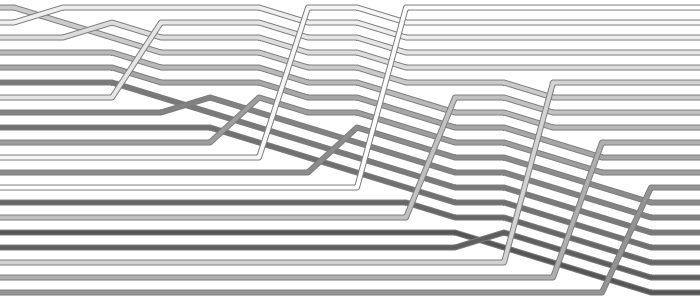
\includegraphics[width=\linewidth]{insertion.png}

  \centerline{Algorithme A.}
\end{minipage}\hfill\begin{minipage}{.49\linewidth}
  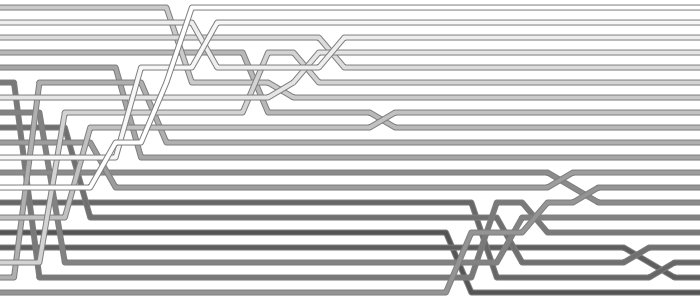
\includegraphics[width=\linewidth]{quick.png}

  \centerline{Algorithme B.}
\end{minipage}

\noindent\begin{minipage}{.49\linewidth}
  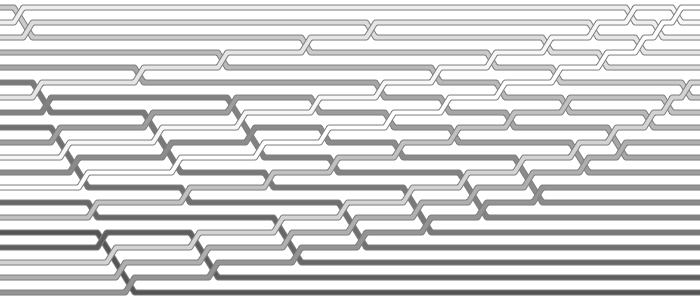
\includegraphics[width=\linewidth]{bubble.png}

  \centerline{Algorithme C.}
\end{minipage}\hfill\begin{minipage}{.49\linewidth}
  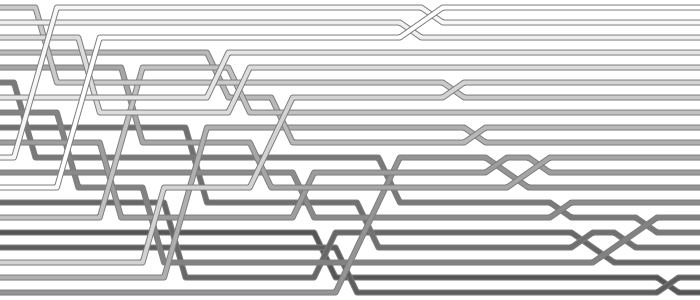
\includegraphics[width=\linewidth]{shell.png}

  \centerline{Algorithme D.}
\end{minipage}

\begin{center}
  \begin{minipage}{.49\linewidth}
    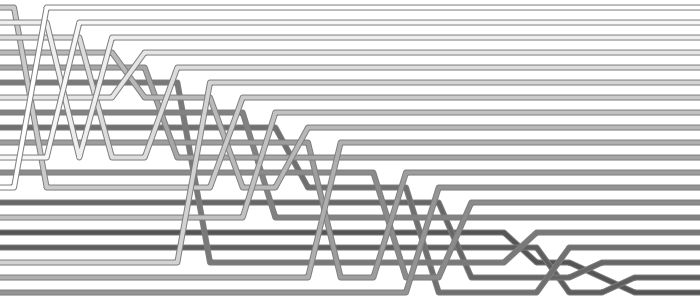
\includegraphics[width=\linewidth]{selection.png}

    \centerline{Algorithme E.}
  \end{minipage}
\end{center}

\begin{Reponse}
  \textbf{Tri a bulle:} parcours successifs du tableau en comparant les voisins
  2 à 2. S'ils sont mal triés, on les inverse. Ce comportement a tendance à
  pousser les grosses valeurs vers la fin. On peut reconnaitre ce comportement
  dans l'algorithme C.

  \textbf{Tri par insertion:} invariant: ce qui est avant la frontière est
  trié. A chaque étape, je prend l'élément juste après la frontière, et je le
  met à sa place dans la partie déjà triée. On peut reconnaitre ce comportement
  dans l'algorithme A.

  \textbf{Tri par selection:} a chaque étape, je selectionne le minimum de la
  partie non triée et le pose à la frontière. On reconnait l'algorithme E.

  \textbf{Shell sort:} comme un bubble sort, mais on commence par trier avec un
  écartement supérieur à 1. Au lieu d'inverser des voisins, on inverse des
  cases à distance 3 puis 2 puis on fait un bubble standard, mais sur un
  tableau un peu prétrié. C'est l'algorithme D.

  \textbf{Quick sort:} c'est un algorithme récursif qui trie une partie du
  tableau puis l'autre (les parties ne sont pas forcément de taille
  identique). C'est l'algorithme B.
\end{Reponse}

\bigskip
\noindent\hspace{-1.3em}$\bigstar$\textbf{Annexe:} Règles de calcul des
préconditions. 

\begin{itemize}
\item \WP{nop, Q}  $\equiv Q$
\item \WP{x:=E, Q} $\equiv Q[x:=E]$
\item \WP{C;D, Q}  $\equiv$ \WP{C, \WP{D,Q}}
\item \textbf{WP}(\texttt{if} $Cond$ \texttt{then} $C$ \texttt{else} $D$,$Q$)
  $\equiv (Cond=\mathtt{true}\Rightarrow \mathbf{WP}(C,Q))~\wedge~
          (Cond=\mathtt{false}\Rightarrow \mathbf{WP}(D,Q))$
\item \textbf{WP}(\texttt{while} $E$ \texttt{do} $C$ \texttt{done} \{inv I var
  V\},Q)  $\equiv I$ ~~;~~  Obligations de preuve:
  \begin{enumerate}
  \item[$\bullet$] $(E=\mathtt{true}\wedge I\wedge V=z) \Rightarrow
    \mathbf{WP}(C,I\wedge V<z))$
  \item[$\bullet$] $I\Rightarrow V\geq 0$
  \item[$\bullet$] $(E=\mathtt{false}\wedge I) \Rightarrow Q$
  \end{enumerate}
\end{itemize}


\end{document}


%%% Local Variables:
%%% coding: utf-8
